\chapter{图模型背景}

我们从图模型的研究背景开始讲解。
最关键的想法是因子分解:一个图模型由可以根据图结构进行因子分解的一系列概率分布构成。
这里的“分布”是不精确的,$p$ 应该被理解为是一个离散的质量函数(计数测度上的密度),或者是连续情况下勒贝格测度的密度。
本章节主要讲解条件独立性(Conditional independence)等概率概念与团(Cliques)、分割(Separation)等图论概念之间的相互关系。

\section{图结构表示的概率分布}

我们首先描述几类有用的图形式。
一个图 $G = (V, E)$ 是由一系列顶点 $V = \{1, 2, \dots, m\}$ 和一系列连边 $E \subset V \times V$ 构成的。
每一条边都连接一对顶点 $s, t \in E$,无向边代表 $(s, t)$ 和 $(t, s)$ 之间并没有什么不同,而有向边可以写为 $(s \rightarrow t)$ 来表达方向。
附录 A.1 有关于图及其性质更多的介绍。

为了定义一个图模型,我们把每个节点 $s \in V$ 都赋予一个从某个空间 $\mathcal{X}_s$ 中取值的随机变量 $X_s$。
取决于具体的应用情况,状态空间 $\mathcal{X}_s$ 既可以是连续的($\mathcal{X}_s = \mathbb{R}$)也可以是离散的($\mathcal{X}_s = \{0, 1, \dots, r-1\}$)。
我们使用小写字母($x_s \in \mathcal{X}_s$)来表示 $\mathcal{X}_s$ 中的特定元素,因此 $\{X_s = x_s\}$ 代表随机变量 $X_s$ 取值为 $x_s \in \mathcal{X}_s$ 的事件。
对于任意的节点子集 $A \subset V$,我们定义子集随机向量 $X_A \coloneqq (X_s, s \in A)$,其对应的取值向量可以表示为 $x_A \coloneqq (x_s, s \in A)$。
同样地,我们定义 $\otimes_{s \in A}\mathcal{X}_s$ 为 $X_A$ 中每个元素状态空间的笛卡尔积。

\subsection{有向图模型}

给定一个带有边 $(s \rightarrow t)$ 的有向图,我们称 $t$ 是 $s$ 的一个子节点,或者相对地,$s$ 是 $t$ 的一个父节点。
对于任意节点 $s \in V$,它的所有父节点构成的集合表示为 $\pi(s)$。
(如果节点 $s$ 没有父节点,那么 $\pi(s)$ 代表空集。)
一个有向环是指一条序列 $(s_1, s_2, \dots, s_k)$,其中对于 $i = 1, \dots, k-1$ 都有 $(s_i \rightarrow s_{i+1}) \in E$,并且 $(s_k \rightarrow s_1) \in E$。
图 \ref{fig:2-1} 对这些概念进行了直观解释。

\begin{figure}[htbp]
    \centering
    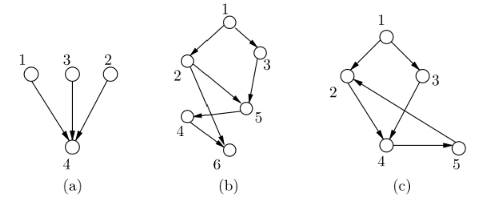
\includegraphics[width=.8\linewidth]{2-1.PNG}
    \caption{
        (a) 一个简单的带有四个变量 $(X_1, X_2, X_3, X_4)$ 的有向图模型。
        节点 $\{1, 2, 3\}$ 是节点 $4$ 的父节点,写作 $\pi(4) = \{1, 2, 3\}$。
        (b) 一个更复杂的有向无环图,定义了其节点的一个偏序(Partial order)结构。
        注意到节点 $6$ 是节点 $2$ 的一个子节点,节点 $1$ 是节点 $6$ 的一个祖先(Ancestor)。
        (c) 一个禁忌的有向图模型(带有环),其中包含了一个有向环路 $(2 \rightarrow 4 \rightarrow 5 \rightarrow 2)$。
    }\label{fig:2-1}
\end{figure}

假设 $G$ 是一个有向无环图(Directed acyclic graph,DAG),这意味着所有的连边都是有向的,并且图上不含有向环路。
对于任意一个 DAG,我们可以通过祖先的概念定义节点集 $V$ 的一个偏序结构:如果存在一条有向路径 $(s, t_1, t_2, \dots, t_k, u)$,则称节点 $s$ 是节点 $u$ 的一个祖先(见图 \ref{fig:2-1}(b))。
给定一个 DAG,对于每一个节点 $s$ 和它的父节点 $\pi(s)$,以 $p_s(x_s|x_{\pi(s)})$ 表示一个定义在变量 $(x_s, x_{\pi(s)})$ 上的非负函数,并且满足归一化条件 $\int p_s(x_s|x_{\pi(s)})dx_s = 1$。
就这些局部函数而言,有向图模型由一系列概率分布(密度或质量函数)组成,这些概率分布可以按照以下方式进行分解:

\begin{equation}
    p(x_1, x_2, \dots, x_m) = \prod_{s \in V}p_s(x_s|x_{\pi(s)})
\end{equation}

在这里,符号的使用与一般习惯是一致的,事实上 $p_s(x_s|x_{\pi(s)})$ 就代表着由因子分解 (2.1) 所表示的分布 $p(\cdot)$ 在给定 $\{X_{\pi(s)} = x_{\pi(s)}\}$ 的情况下 $\{X_s = x_s\}$ 的条件概率。
这是一个可以利用 $p_s(\cdot)$ 的归一化条件和 DAG 上由祖先关系导出的偏序结构所得到的归纳结论。

\subsection{无向图模型}

在无向的情形下,概率分布可以根据定义在图上的团(Cliques)结构进行因子分解。
一个团 $C$ 是指节点集 $V$ 的一个全连接子集,意味着对于所有 $s, t \in C$ 都有 $(s, t) \in E$。
我们在每个团结构 $C$ 上都定义一个势函数(Compatibility function) $\psi_C: (\otimes_{s \in C}\mathcal{X}_s) \rightarrow \mathbb{R}_+$。
注意 $\otimes_{s \in C}\mathcal{X}_s$ 表示随机向量 $X_C$ 状态空间的笛卡尔积。
因此势函数 $\psi_C$ 是一个仅仅定义在团元素上的局部量。

使用这些记号一个无向图模型——或者说马尔可夫随机场(Markov random field, MRF),又或者说吉布斯分布(Gibbs distribution)——是一系列能够进行以下分解的分布:

\begin{equation}
    p(x_1, x_2, \dots, x_m) = \frac{1}{Z}\prod_{C \in \mathcal{C}}\psi_C(x_C)
\end{equation}

其中 $Z$ 是归一化常数。
$\mathcal{C}$ 经常取为图上所有的最大团(Maximal cliques)组成的集合,也就是不属于任何其他团的团所构成的集合。
这个条件可以保证不失一般性,因为任何基于非最大团的表示总是可以转化为基于最大团的表示,只需要重新定义最大团上的势函数,使之成为该团子集上的势函数的乘积即可。
然而,使用非最大团的表示可能带来计算的简便性,尤其是在算法可以利用基于非最大团的因子分解的特点的时候。
因此,我们不必将势函数限制在最大团上,而是将集合 $\mathcal{C}$ 定义为可以包含任何团结构。
(在下一节讨论的因子图将会对分解属性提出更细致的规范。)

必须理解的是,对于一个一般的无向图而言,势函数 $\psi_C$ 并不需要与定义在团上的边缘或条件分布有任何明显或直接的关系。
这个属性与有向图的因子分解形成了对比,在有向图中因子对应着父子节点之间的条件概率。

\subsection{因子图}

对于大规模的图而言,无论是有向图还是无向图,它的因子分解都很难从图的通常描述中观察得到。
因子图(Factor graphs)的形式提供了图的另一种表示方法,主要强调对分布的分解。

令 $F$ 为定义在图模型分布上的因子的索引集。
在无向图的情况下,$F$ 索引了 $\mathcal{C}$ 中的团结构,在有向图的情况下则索引了父子节点集。
接下来我们考虑一个二分图 $G' = (V, F, E')$,其中 $V$ 还是原来的节点集合,$E'$ 是一个新的边集合,连接节点 $s \in V$ 和因子 $a \in F$。
特别地,$(s, a) \in E'$ 当且仅当 $x_s$ 存在于由 $a \in F$ 索引的因子中。
参见图 \ref{fig:2-2}(b)。

\begin{figure}[htbp]
    \centering
    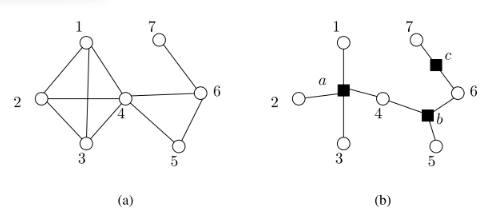
\includegraphics[width=.8\linewidth]{2-2.PNG}
    \caption{
        无向图和因子图。
        (a) 7个节点上的无向图,拥有最大团 $\{1, 2, 3, 4\}$,$\{4, 5, 6\}$ 和 $\{6, 7\}$。
        (b) (a) 中无向图等价的因子图表示,假设我们只在最大团上定义了势函数。
        因子图是一个二部图,拥有节点集 $V = \{1, \dots, 7\}$ 和因子集 $F = \{a, b, c\}$,每个因子对应原无向图上的一个势函数。
    }\label{fig:2-2}
\end{figure}

对于无向图模型来说,当 $\mathcal{C}$ 包含不仅仅只是最大团时,因子图表示具有特殊的价值。
事实上在一般的无向图表示中,非最大团的势函数并没有明显的表示出来,而因子图可以让它们显性化。

\section{条件独立性}

由式 (2.1) 和式 (2.2) 定义的概率分布族在随机变量的子集之间存在着条件独立性的特征——原图模型的马尔可夫性(Markov properties)。
我们在这里只粗略过一下这个特性,因为在文章其他部分并没有涉及到太多相关的内容。
如果读者对此有兴趣,我们推荐可以去看一下 Lauritzen 的作品。

对于无向图模型而言,条件独立性与图论中的可达性概念相一致。
特别地,令 $A$,$B$ 以及 $C$ 是互不相交的节点子集三元组。
如果删掉节点集 $C$ 之后没有任何一条路径能够从 $A$ 到达 $B$,那么我们称在给定 $X_C$ 的条件下 $X_A$ 与 $X_B$ 是独立的。
在子集 $A$,$B$ 以及 $C$ 的所有可能选择范围内可以产出一个条件独立性列表。
这些列表总是自洽的(即存在满足这些列表中所有条件独立性的概率分布),而且符合条件的概率分布集正是由式 (2.2) 所定义的分布集,涵盖了势函数的所有可能选择。

因此与无向图相关的概率分布族有两种等价刻画。
这个等价性是一个基本的数学结论,连接了一个代数概念(因子分解)和一个图论概念(可达性)。
这一结论也产出了一个可以用来检验条件独立性的算法,因为它将条件独立性的评估问题简化为图上可达性的评估问题。
这很容易用图上的广度优先搜索来解决。

在有向图模型中也有类似的结果,唯一的变化是可达性的概念。
同样,在有向图的因子分解 (2.1) 中指定的概率分布族与根据一组条件独立性所定义的概率分布族之间建立等价关系是可能的。

\section{统计推断和精确算法}

给定一个定义在图模型上的概率分布 $p$,我们主要关注解决以下一个或多个计算推断问题(Computational inference problems):

\begin{enumerate}
    \item[(1)] 计算观测得到的数据的似然。
    \item[(2)] 计算特定子集 $A \subset V$ 的边缘分布 $p(x_A)$。
    \item[(3)] 计算不相交子集 $A$ 和 $B$ 的条件分布 $p(x_A|x_B)$。
    \item[(4)] 计算密度的众数($\hat{x} = arg\max_{x \in \mathcal{X}}p(x)$)。
\end{enumerate}

显然问题 (1) 是问题 (2) 的一个特例。
(3) 中条件概率的计算似乎也是需要边缘化的步骤,首先需要得到分子 $p(x_A, x_B)$,然后需要得到分母 $p(x_B)$。
相较而言,(4) 中关于众数的计算从基础上就是不同的,因为它涉及最大化而不是积分的问题。
尽管如此,我们后续所提出的变分方法将会突出某些计算边际与计算众数的重要联系。

为了理解这些推断问题的内在挑战,考虑一个离散随机向量的例子 $x \in \mathcal{X}^m$,其中对于每个节点 $s \in V$ 都有 $\mathcal{X}_s = \{0, 1, \dots, r-1\}$。
在单个节点上计算边际 $p(x_s)$,一种朴素的方法是对所有的 $\{x' \in \mathcal{X}^m|x_s' \neq x_s\}$ 进行求和。
这个集合一共有 $r^{m-1}$ 个元素,很明显很难用暴力方法来处理这种问题。
即使是二元变量($r = 2$)和一个 $m \approx 100$ 个节点的图(对于很多应用程序来说规模很小),这个求和也超出了暴力计算的能力范围。
类似地,在这个离散地情况下计算一个众数需要在一个指数量级地可行解空间解决一个整数规划问题。
对于连续随机变量,问题并不会得到简化 \footnote{高斯情况是一个特例} 而通常会更难,因为它们需要计算大量的积分。

对于没有环的无向图和每个节点只有一个父节点的有向图——也就是树——来说,这些推断问题都能够利用自然的动态规划性质使用“消息传递(Message-passing)”递归算法得到精确的解决,计算复杂度只是节点数量的线性量级。
特别地,在计算边际的情况下,动态规划将会退化为另一种一般算法的形式,称为和积算法(Sum-product),而对于计算众数的问题则退化为另一种相似的最大积算法(Max-product)。
我们将在 2.5.1 小节描述这些算法。
更一般地说,正如我们将在 2.5.2 小节中讨论的,联合树算法(Junction tree)为任意图的推断问题提供了一种解决方案。
联合树算法的计算复杂度的指数级的,底数为图的树宽(Treewidth)。

\section{应用}

在转向算法问题的研究之前,我们最好先广泛地讨论一下各种图模型的应用实例。
我们展示了几个一般场景下的图模型应用实例,包括贝叶斯层次建模、列联表分析、组合优化和可满足性等一般领域中使用图模型的例子,以及在生物信息学、语音和语言处理、图像处理、空间统计、通信和编码理论中的具体例子。

\subsection{贝叶斯层次建模}

贝叶斯框架把所有模型量都作为随机变量,包括观测数据、隐变量、参数、干扰变量等。
因此图模型表示下的贝叶斯模型,所有这些变量都以节点的身份出现在图中。
与图模型相关的通用计算方法可以直接应用于参数的边际和后验概率等贝叶斯量的计算。
尽管贝叶斯模型能够使用有向或无向图两种进行表示,实践中所遇到的大多数还是以有向图为主。
特别地,在贝叶斯层次模型中,先验分布的定义通常涉及额外的参数,称为超参数,而整个模型被定义为一组连接超参数、参数和数据的条件概率。
把这些条件概率分布做乘积就得到了联合概率分布,这种因子分解只是式 (2.1) 的一个简单实例而已。

把贝叶斯层次模型当作有向图模型看待有几点好处。
第一,层次模型通常通过对条件独立性的各种说明来指定。
这些说明暗含了其他条件独立性关系,而且可达性算法也提供了一种系统性的方法来验证这些关系。
第二,由图提供的可视化既能帮助理解模型(包括验证图无环的基本步骤),也更有利于进行扩展和探索。
最后,一般的计算方法如 MCMC 和变分推断算法等都能够应用在图模型上,因此就需要把层次模型表达为图的形式。
这些方便之处促进了通过有向图形式来操作贝叶斯层次模型的通用软件程序的发展。

\subsection{列联表分析}

列联表是一种应用于多类型数据分析中的核心工具,可以追溯到 Pearson、Yule 和 Fisher 的开创性研究。
一个 $m$ 维的,每个维度都有 $r$ 个水平的列联表表示一个定义在 $m$ 个随机变量 $(X_1, \dots, X_m)$,每一个随机变量都有 $r$ 个可能取值的概率分布。
举个具体的例子 $m = 2$,一个具有 $r$ 个水平的列联表是一个简单的 $r \times r$ 的元素非负的加和为 $1$ 的矩阵,对于 $m > 2$ 来说则是一个具有 $r^m$ 个非负元素且加和为 $1$ 的多维数组。
因此,这个表完整地确定了一个定义在随机向量 $(X_1, \dots, X_m)$ 上的,每个随机变量 $X_s$ 取 $r$ 个可能取值的概率分布。

列联表可以使用图模型的框架进行建模,而且图的形式给许多自然的问题提供了一种很有帮助的可视化。
例如,在列联表分析中一个核心问题是区分数据中不同的交互顺序。
作为一个具体的例子,给定 $m = 3$ 个变量,一个简单的问题是测试这三个变量之间是否独立。
从图模型的角度来看,这个测试相当于在相关的交互图上连接是否是全部断开的(见图 \ref{fig:2-3}(a)(b))。
一个更微妙的测试是区分随机变量是否仅以成对的方式相互作用(用式 (2.2) 来说就是只有因子 $\psi_{12}$,$\psi_{13}$ 以及 $\psi_{23}$),又或者实际上是三方交互作用(式 (2.2) 中仅有 $\psi_{123}$)。
有趣的是这两种因子分解的方式是没办法用标准的无向图来进行区分的,如图 \ref{fig:2-3}(b) 所示,3 个节点的全连接图是不区分三重交互作用与成对交互作用的。
这么看来因子图的形式更为有效,因为它是能够区分成对交互和三重交互的,如图 \ref{fig:2-3}(c)(d) 所示。

\begin{figure}[htbp]
    \centering
    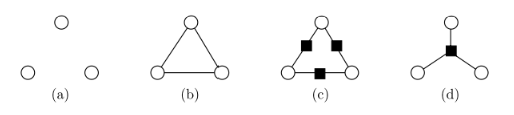
\includegraphics[width=.8\linewidth]{2-3.PNG}
    \caption{
        列联表分析中一些简单的图交互作用。
        (a) 独立模型。
        (b) 一般的非独立模型。
        (c) 只有成对交互作用。
        (d) 三重交互作用。
    }\label{fig:2-3}
\end{figure}

\subsection{约束满足和组合优化}

约束满足和组合优化问题出现在各种各样的领域,其中包括人工智能、通信理论、计算复杂性理论、统计图像处理和生物信息学。
可满足性和组合优化中的许多问题都是用图论的术语定义的,因此很自然地以图模型的形式进行重塑。

让我们考虑一个可能是最著名的可满足性的例子,即 3-SAT 问题。
它可以很自然地用因子图和二元随机变量 $(X_1, X_2, \dots, X_m) \in \{0, 1\}^m$ 来表示。
对于一个给定的节点三元组 $\{s, t, u\}$,我们首先定义一些“禁忌”的模式 $(z_s, z_t, z_u) \in \{0, 1\}^3$,然后再定义三元组的势函数

\begin{equation}
    \psi_{stu}(x_s, x_t, x_u) = \begin{cases}
        0 & \text{如果} (x_s, x_t, x_u) = (z_s, z_t, z_u) \\
        1 & \text{其他}
    \end{cases}
\end{equation}

每个这样的势函数在可满足性的文献中被称为子句,通常按照逻辑操作进行编码。
举个具体的例子,如果 $(z_s, z_t, z_u) = (0, 0, 0)$,那么式 (2.3) 就能被简洁地写为 $\psi_{stu}(x_s, x_t, x_u) = x_s \vee x_t \vee x_u$,其中 $\vee$ 代表两个布尔符号间的逻辑或操作。

作为一个图模型,图 \ref{fig:2-3}(d) 和一个单子句相关,让人更感兴趣的是建立在更大规模的二元变量集之上的模型,其中包含许多子句。
在可满足性上的一个基本问题是判断给定的一个子句集合 $F$ 是否是可满足的,这意味着存在某种配置 $x \in \{0, 1\}^m$ 使得 $\prod_{(s, t, u) \in F}\psi_{stu}(x_s, x_t, x_u) = 1$。
在这种情况下,因子分解 $$p(x) = \frac{1}{Z}\prod_{(s, t, u) \in F}\psi_{stu}(x_s, x_t, x_u)$$ 定义了在满足的配置集合上的均匀分布。

如果 3-SAT 的实例是随机构建的——例如固定一个子句密度 $\alpha > 0$,然后从 $m$ 个变量组成的三元组中随机抽取 $\lceil\alpha m \rceil$ 个子句——图的形式将会趋向于一种局部的“类树”结构,参见图 \ref{fig:2-9}(b)。
这个问题上存在一个临界点 $\alpha^*$,当 $\alpha$ 小于这个值的时候基本没什么约束,而当 $\alpha$ 足够大的时候基本就是不可满足的,这种相变的现象是相关研究中的一个重要问题。

调查传播算法(Survey propagation)是解决随机可满足性问题的一种很有前景的方法,它是从统计物理领域发展起来的。
已经有研究表明调查传播算法是和积算法或者信念传播算法在以图模型表示的可满足性问题上的一个特例。

\subsection{生物信息学}

生物信息学中的许多经典模型都是图模型的实例,图模型的相关框架也常被用来设计新的模型。
本小节我们简单回顾一些在生物信息学中所应用到的经典的或者最近的图模型例子。
序列数据在生物信息学领域有着十分重要的地位,图 \ref{fig:2-4}(a) 所示的隐马尔可夫模型(Hidden markov model, HMM)是对序列数据进行处理的一个基础模型。
HMM 本质上是有限混合模型的一个动态版本,这类模型都假设观测数据是在一个隐状态下产生的。
状态变量通常是服从多项式分布的离散随机变量,在时序上构成马尔可夫链。
图 \ref{fig:2-4}(a) 表示的图模型同样也是基于卡尔曼滤波(Kalman filter)的状态—空间模型(State-space model),这个模型下的状态变量是一个高斯向量。
这个模型同样也可以被称为是“隐马尔可夫模型”,只不过这个名称通常是指状态变量取离散值的模型。

\begin{figure}[htbp]
    \centering
    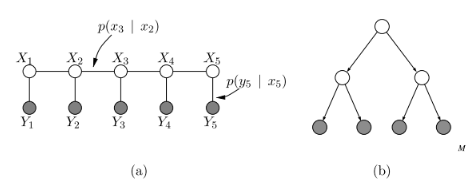
\includegraphics[width=.8\linewidth]{2-4.PNG}
    \caption{
        (a) 一般隐马尔可夫模型的图表示。
        阴影节点 $\{Y_1, \dots, Y_5\}$ 代表观测变量,非阴影节点 $\{X_1, \dots, X_5\}$ 代表隐状态变量。
        后者构成了一条马尔可夫链,在给定 $X_t$ 的条件下 $X_s$ 独立于 $X_u$,其中 $s < t < u$。
        (b) 在四个现存的有机体和 $M$ 位点上的物种演化的图表示。
        这棵树诠释了这么一种假设:首先有一个物种形成事件,随后有两个进一步的物种形成事件,最终形成了现存的四种生物。
    }\label{fig:2-4}
\end{figure}

将联合树算法应用到 HMM 上产生了一种新的算法,新算法沿着状态变量链在两个方向上进行消息传递,以此计算边际概率 $p(x_t, x_{t+1}|y)$ 和 $p(x_t|y)$。
这套消息传递算法在 HMM 中被称为前后向算法(Forward-backward algorithm)。
这些边际概率的推断过程本身很有趣,而在对 HMM 进行参数估计的时候,这些边际概率在所使用的期望最大化(Expectation-maximization,EM)算法中也扮演着充分统计量的重要作用。
类似地,最大后验状态序列也能通过联合树算法计算出来(用最大化代替求和)——这个算法在 HMM 中被称为维特比算法(Viterbi algorithm)。

基因发现是 HMM 的一个应用场景。
粗略地说,一个有机体的基因组序列可以分为包含基因的区域和基因间的区域(分离基因),其中基因作为一段核苷酸序列,可以进一步地分为有意义的基因内结构(外显子和内含子)。
这些区段之间的边界是高度随机的,因此很难可靠地把它们找出来。
HMM 是解决这一问题的方法之一,设计者可以将有关基因结构的生物学知识编码进状态和状态转移过程。
HMM 也可以用来为蛋白质结构进行建模。
例如,膜蛋白是一种特殊的蛋白质,它们嵌入到细胞膜中,在细胞内外信号的传递中起着重要的作用。
这些蛋白质多次进出细胞膜,在亲水基性氨基酸和疏水基性氨基酸之间交替。
这些生物学知识被用来设计跨膜 HMM(一种建模膜蛋白的 HMM 模型)的状态和状态转移矩阵。

树结构模型在生物信息学和语言处理中也发挥着重要作用。
例如物种演化树可以看作图模型。
如图 \ref{fig:2-4}(b) 所示,物种演化树是一种树结构的图模型,其中一组观察到的核苷酸(或者其他生物学特征)假定是从一组潜在的祖先物种进化而来。
树中的条件概率是通过进化替代模型得到的,而可能性的计算是通过在树上进行递归剪枝来实现的。
这种递归是联合树算法的一个特例。

图 \ref{fig:2-5} 展示了一些在生物信息学中被应用的更为复杂的图模型。
图 \ref{fig:2-5}(a) 展示了隐马尔可夫物种演化模型,其中观察到的是一组与物种演化树相关的核苷酸。
基于多种灵长类动物的数据,这一模型已被证明对人类基因组的基因发现很有作用。
图 \ref{fig:2-5}(b) 展示了因子隐马尔可夫模型,其中多个链通过与一组共同的观察变量相连接而耦合。
这个模型抓住了遗传学中的多位点连锁分析的问题,其中状态变量对应于减数分裂时染色体上的相位。

\begin{figure}[htbp]
    \centering
    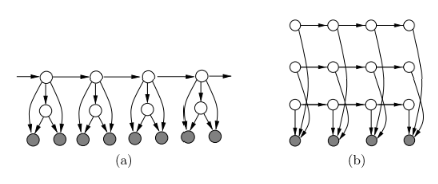
\includegraphics[width=.8\linewidth]{2-5.PNG}
    \caption{
        应用在生物信息学上的 HMM 的变体。
        (a) 物种演化 HMM。
        (b) 因子 HMM。
    }\label{fig:2-5}
\end{figure}

\subsection{语言和语音处理}

在语言问题中,HMM 也扮演着一种基础角色。
一个例子就是词性问题,把句子中的单词标注它们的词性(名词、动词、形容词等)。
其中状态变量为语料库的词性,转移矩阵可以通过 EM 算法进行估计。
在一个新句子上运行维特比算法是根据句子中单词的假设词性对句子进行标注。
此外,基本上所有的现代语音识别系统都建立在 HMM 的基础上。
在这种情况下,观察到的通常是一系列短程语音谱,而状态则对应于如音素或者音素对等间隔的语音单元。
大规模系统是通过将基本的 HMM 进行组合而得到更大的图模型来构建的。

图 \ref{fig:2-6}(a) 所示的图模型是一个耦合的 HMM,其中两个状态变量链通过连边耦合,该模型适用于语音识别中音频和唇语数据对的融合。
图 \ref{fig:2-6}(b) 展示了一种 HMM 变体,其中状态相关的观测变量分布是一个有限混合模型。
这种变体被广泛应用在语音识别系统中。

\begin{figure}[htbp]
    \centering
    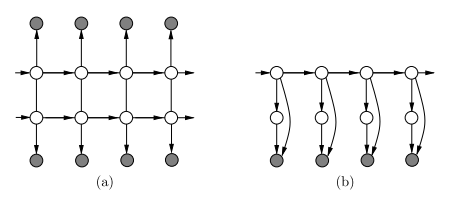
\includegraphics[width=.8\linewidth]{2-6.PNG}
    \caption{
        HMM 在语言和语音处理中的拓展。
        (a) 耦合 HMM。
        (b) 带有混合模型的 HMM。
    }\label{fig:2-6}
\end{figure}

另一类在语言处理中被广泛研究的模型叫“词袋(Bag-of-words)”模型,尤其在大规模文档语料建模中很常见。
词袋的意思是假设文档中单词的顺序不重要,亦即假设了单词位置的可交换性。
这些模型的目标通常是在语料库中找到潜在的“主题”,并利用这些主题对文档进行聚类或者分类。
词袋模型的一个实例是隐迪利克雷分配(Latent Dirichlet Allocation, LDA),在这个模型中,主题是定义在单词上的概率分布,文档是定义在主题上的概率分布。
特别地,如图 \ref{fig:2-7} 所示,语料库中的每篇文档都假设是通过采样一个带有超参数 $\alpha$ 的 Dirichlet 变量,然后根据这些 Dirichlet 概率反复选择一个主题,并从与所选主题相关的分布中选择一个单词来生成的 \footnote{这个模型将会在 3.3 小节中的例 3.5 进行详细讲解。}。

\begin{figure}[htbp]
    \centering
    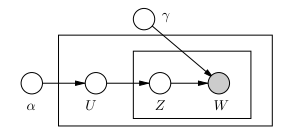
\includegraphics[width=.5\linewidth]{2-7.PNG}
    \caption{
        LDA 的图模型表示。
        变量 $U$ 遵从参数为 $\alpha$ 的 Dirichlet 分布,“主题”变量 $Z$ 遵从参数为 $U$ 的多项分布。
        “单词”变量 $W$ 同样是基于 $Z$ 的多项分布,$\gamma$ 指定与每个主题相关的单词概率。
        这些矩形称作盘子(Plates),在矩形内部的随机变量是保持条件独立性进行重复的。
    }\label{fig:2-7}
\end{figure}

\subsection{图像处理和空间统计}

几十年来,无向图模型或马尔可夫随机场在图像处理和更一般的空间统计中发挥了重要作用。
对于图像建模,最简单的马尔可夫随机场是在像素域,图像中的每个像素都与底层图中的一个节点相关联。
还有很多其他的结构化模型是建立在每个空间位置的特征向量上的,其中每个特征可以是一个线性多尺度滤波器(如小波)或者更复杂的非线性算子。

对于图像建模,一个最自然的图结构是 2D 网格,例如图 \ref{fig:2-8}(a) 中所示 4-最近邻网络。
通常选择相邻像素(或者更一般的特征)连边上的势函数来表示局部平滑条件。
图像处理的各种任务,包括去噪、分割和超分辨率等,都需要在这样的马尔可夫随机场上解决相应的推断问题。
然而对于大规模格点模型的精确推断是很难的,因此需要近似算法。
MCMC 方法被用得很多,但是对于很多应用来说计算量可能太大,速度不够快。
最近诸如和积算法与树重加权(Tree-Reweighted)最大积算法等消息传递算法已成为图像处理和计算机视觉问题的一种近似推断方法。

另一种策略是用一个更简单的——近似的——模型来代替格点模型,从而避开格点模型的难处。
例如多尺度 4 叉树,如图 \ref{fig:2-8}(b) 所示,就能用来近似格点模型。
这种多尺度模型的优点是允许利用高效的树算法来进行精确推断。
然而带来的问题是模型不完美,可能会导致图像重构中出现伪影。

\begin{figure}[htbp]
    \centering
    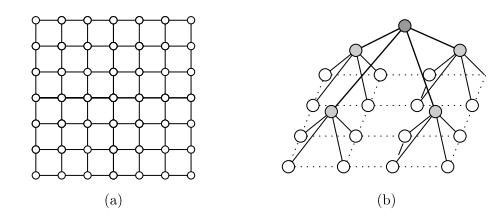
\includegraphics[width=.8\linewidth]{2-8.PNG}
    \caption{
        (a) 2D 的 4-近邻网格模型经常被用来做图像建模。
        (b) 多尺度的 4 叉树 2D 格点近似模型。
        原始格点(白色)对应的节点位于树的最小尺度上。
        树的中部和顶部尺度由辅助节点构成(灰色),引入辅助节点对精细尺度行为进行建模。
    }\label{fig:2-8}
\end{figure}

\subsection{纠错编码}

通信理论的核心问题是把信息以比特序列的形式从一点传送到另一点。
例如个人计算机在网络上的通信或者从卫星到地面的通信等。
如果通信信道是有噪声的,那么某些传输位可能被损坏。
为了对抗这种噪声,一种自然的策略是给传输的比特序列添加冗余,从而定义编码字。
原则上,这种编码策略允许在存在一些错误的情况下完美地解码通信。

现在使用的很多最好的编码,包括 Turbo 码和低密度奇偶校验码,都是基于图模型的。
图 \ref{fig:2-9}(a) 展示了一个非常小的奇偶校验码的因子图形式。
(图 \ref{fig:2-9}(b) 展示了更大的编码)。
在左边,6 个白色节点代表组成编码字 $x_i$(也就是长度为 6 的二元序列),而灰色节点代表与这些比特序列相关的噪声观测结果 $y_i$。
在右边,每个黑色方块节点代表一个因子 $\psi_{stu}$,表示三元组 $\{x_s, x_t, x_u\}$ 的奇偶性。
该奇偶关系在数学上表示为 $x_s \oplus x_t \oplus x_u \equiv z_{stu}$ 的模二算法,可以用如下形式的势函数表示为无向图模型:
$$\psi_{stu}(x_s, x_t, x_u) \coloneqq \begin{cases}
    1 & \text{如果} x_s \oplus x_t \oplus x_u = 1 \\
    0 & \text{其他}
\end{cases}$$
对于图 \ref{fig:2-9} 所示的编码,奇偶校验范围在三元组 $\{1, 3, 4\}$、$\{1, 3, 5\}$、$\{2, 4, 6\}$ 和 $\{2, 5, 6\}$ 的集合上。

解码问题需要根据噪声观测的向量 $y = (y_1, y_2, \dots, y_m)$ 来估计传输的是哪个编码字。
有了信道噪声模型的表示,这个解码问题可以归结为一个推断问题。
根据损失函数,最佳解码要么基于每个节点边际概率 $p_s(x_s = 1|y)$ 计算,要么直接计算最可能的编码字(即后验的众数)。
对于图 \ref{fig:2-9}(a) 的简单编码,通过联合树算法可以很容易实现最优解码。
然而在很多应用中人们感兴趣的是比特数很容易达到几千位的大规模编码。
这些编码下的图模型有着很大的树宽值,因此联合树算法不可行。
此外 MCMC 算法在该领域也还没有得到成功的应用。

\begin{figure}[htbp]
    \centering
    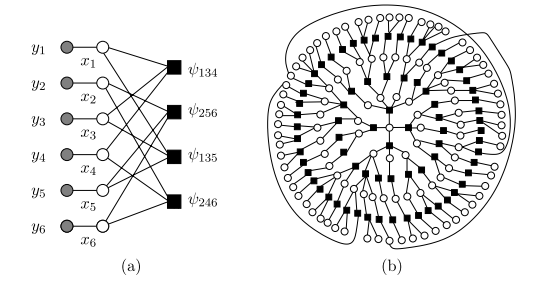
\includegraphics[width=.8\linewidth]{2-9.PNG}
    \caption{
        (a) 长度为 $m = 6$ 的奇偶校验码的一种因子图表示。
        在左边,圆形的白色节点代表定义编码的未观测比特位 $x_i$,而圆形的灰色节点代表从通道接收到的观测值 $y_i$。
        在右边,黑色方块代表相关的因子,或奇偶校验。
        这个特定的编码是 $(2, 3)$ 码,因为每个比特都与两个奇偶性变量相连,每个奇偶性关系涉及三个比特。
        (b) 具有“局部树状”结构的大型因子图。
        $m$ 个有界度节点上的因子图的随机构造具有典型长度 $\log{m}$ 的环,这种树状属性可以大大促进近似解码的和积算法的成功应用。
    }\label{fig:2-9}
\end{figure}

对于许多图编码,最成功的解码器是基于和积算法的,2.6 小节将对其进行详细讨论。
由于定义好的编码的图模型总是有环,和积算法不能保证计算出正确的边际,甚至有可能不能收敛。
尽管如此,这种近似解码算法对于大规模的编码来说还是有非常积极的意义。
和积算法在编码长度趋向于无穷的情况下是很容易理解的,可以使用鞅参数来证明收敛结果。
相较之下对于一般长度的编码就不那么好理解了。

\section{精确推断算法}

本节我们开始讲解图模型的基本精确推断算法。
在计算边际概率的时候,我们必须在一个或多个变量上对联合概率分布进行求和或者积分。
我们可以通过选择特定的变量顺序把这个计算过程表示为一个操作序列(可以利用 Fubini 定理)。
回想一下无论是有向还是无向图模型,联合概率都是变量子集的因子表达式。
因此我们可以充分利用分配律,调整求和或积分与乘积的顺序。
“精确推断”指的是组织计算顺序的问题,同时也需要对中间过程出现的新因子进行管理。
假设每个单独的求和或积分都计算得很精准,那么整个算法就会给出精确得数值结果。

为了得到单个变量 $X_s$ 的边际概率分布,只需要为其他变量指定一个顺序进行求和或积分消除即可。
对每个单独的变量重复整个过程就能得到完整的边缘集。
然而这种方法是低效的,因为它没有考虑有些中间项是可以在各个不同的边际计算过程中共用的。
和积算法和联合树算法本质上是基于共享中间项的动态规划算法。
算法涉及图结构上的“消息传递”操作,其中的消息就是指的这些可以共享的中间项。
如果算法收敛,我们就可以得到原图模型上所有团的边际概率。

有向图和无向图模型都涉及到联合概率分布的因子表达式,因此精确推断算法在本质上以相同的方式对它们进行处理。
实际上为了使得推断算法具有普适性,一般将有向图转换为无向图,并且统一在无向图的模式下进行处理。
我们可以看到有向图的因子分解 (2.1) 并不一定在团上定义,因为给定节点的父节点之间并不一定是连通的。
因此我们将一个有向图转换为一个无向的道德图(Moral Graph),其中每个子节点的父节点间都被连接,所有有向边都转换为无向边。
在这个道德图中,因子都是在团上进行定义的,因此任何有向分解 (2.1) 都是无向分解 (2.2) 的特例。
在这篇文章剩下的部分中,我们假设都已经进行了这种转换。

\subsection{树结构上的消息传递}

我们现在开始讨论用消息传递算法在树结构上进行精确推断。
我们在这里的讲解很简单,读者有兴趣的话可以参考相关的引文。
首先可以看到的是树 $T = (V, E(T))$ 上的团仅仅是单个的节点和边。
因此任何树形结构的图模型都能够进行以下分解:
\begin{equation}
    p(x_1, x_2, \dots, x_m) = \frac{1}{Z}\prod_{s \in V}\psi_s(x_s)\prod_{(s, t) \in E(T)}\psi_{st}(x_s, x_t)
\end{equation}
在这里我们稍微描述一下怎样对树结构的图上的任意节点使用和积算法计算边际概率
\begin{equation}
    \mu_s(x_s) \coloneqq \sum_{\{x'|x_s' = x_s\}}p(x_1', x_2', \dots, x_m')
\end{equation}
我们将重点讨论离散随机变量的情况,连续的情况原则上都可以利用积分替代求和得到。

和积算法:和积算法本质上是非串行动态规划的一种形式,它将确定性动态规划通常的串行形式推广到了任意的树形图。
动态规划(DP)的基本原则是分而治之:通过将一个大问题分解为一系列更简单的问题来进行解决。
在图模型中,树结构本身提供了一种对问题进行分解的自然方法。

对于任意节点 $s \in V$,考虑它的邻居集合
\begin{equation}
    N(s) \coloneqq \{u \in V| (s, u) \in E\}
\end{equation}
对于每个邻居节点 $u \in N(s)$,令 $T_u = (V_u, E_u)$ 为 $u$ 可以不用经过 $s$ 就能够到达的节点集(以及连接它们之间的边)所形成的子图。
树结构的一项关键属性就是这样的子图 $T_u$ 也仍然还是树结构,并且对于 $u \neq v$,$T_u$ 和 $T_v$ 的节点是没有重合的。
这样的话,每一个邻居节点 $u \in N(s)$ 都能被视为子树 $T_u$ 的根节点,如图 \ref{fig:2-10} 所示。

\begin{figure}[htbp]
    \centering
    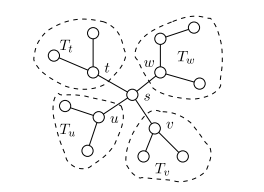
\includegraphics[width=.5\linewidth]{2-10.PNG}
    \caption{
        一棵以 $s$ 为根节点的树的分解。
        节点 $s$ 的每一个邻居节点 $u$ 都是一棵子树 $T_u$ 的根节点。
        在图中移除掉节点 $s$ 之后不同子树之间是不连通的。
    }\label{fig:2-10}
\end{figure}

对于每棵子树 $T_t$,我们定义与其节点变量相关的子向量 $x_{V_t} \coloneqq (x_u, u \in V_t)$。
现在考虑式 (2.4) 中 与子树 $T_t$ 的节点或边的相关的项的集合。
我们把这些项汇总到一起,写成下面的乘积形式:
\begin{equation}
    p(x_{V_t}; T_t) \propto \prod_{u \in V_t}\psi_u(x_u)\prod_{(u, v) \in E_t}\psi_{uv}(x_u, x_v)
\end{equation}
通过这种表示法,树的条件独立性允许将节点 $s$ 的边际计算分解为子问题的乘积,集合 $\{T_t, t \in N(s)\}$ 中每一棵子树都对应一个子问题,具体分解情形如下所示:
\begin{subequations}
\begin{align}
    \mu_s(x_s) &= \kappa\psi_s(x_s)\prod_{t \in N(s)}M_{ts}^*(x_s) \\
    M_{ts}^*(x_s) &\coloneqq \sum_{x_{V_t}'}\psi_{st}(x_s, x_t')p(x_{V_t}'; T_t)
\end{align}
\end{subequations}
上式中 $\kappa$ 为确保 $\mu_s$ 归一化的正数。
对于固定的 $x_s$,子问题定义的 $M_{ts}^*(x_s)$ 同样是一个树结构的求和,只不过这棵子树 $T_t$ 比原来的树 $T$ 小。
因此它也可以采用类似的方式进行递归分解。
这样,节点 $s$ 的边际就可以通过一系列递归更新来计算。

和积算法并不是将上述过程分别应用到每个节点,而是同时并行地计算所有节点地边际。
在每次迭代中,每个节点 $t$ 向它的邻居 $u \in N(t)$ 传递一条“消息”。
我们用 $M_{tu}(x_u)$ 来表示这个消息,它本质上是可能状态 $x_u \in \mathcal{X}_u$ 的一个函数(一个长度为 $|\mathcal{X}_u|$ 的离散随机向量)。
在整个图上一共有 $2|E|$ 条消息,每条边的每个方向上都有一条消息。
整个消息集合根据以下递归规则进行更新
\begin{equation}
    M_{ts}(x_s) \leftarrow \kappa\sum_{x_t'}\{\psi_{st}(x_s, x_t')\psi_t(x_t')\prod_{u \in N(t)/s}M_{ut}(x_t')\}
\end{equation}
其中 $\kappa > 0$ 是一个归一化常数。
可以证明,在树结构图上经过式 (2.9) 的有限次迭代将收敛到唯一的不动点 $M^* = \{M_{st}^*, M_{ts}^*, (s, t) \in E\}$。
所求得的不动点 $M_{ts}^*$ 与式 (2.8b) 中的子问题的解只差一个归一化常数。
由于不动点 $M^*$ 计算出了所有子问题的解,所有节点 $s \in V$ 的边际就可以轻松使用式 (2.8a) 计算出来。

最大积算法:将式 (2.9) 中的求和换成求最大值。
最大积算法可以用来求解树结构分布的众数问题。
在这个意义上可以把它看作是维特比算法从链式结构到树结构的推广。
更进一步地说,最大积算法将收敛到另一个与和积算法不同的唯一的不动点 $M^*$。
通过类比式 (2.7) 这个不动点可以用来计算图中任意节点的最大边际
\begin{equation}
    \nu_s(x_s) \coloneqq \max_{\{x'|x_s' = x_s\}}p(x_1', x_2', \dots, x_m')
\end{equation}
给定这些最大边际可以使用标准的回溯法(Back-tracking)来计算分布的众数 $\hat{x} \in arg\max_{x'}p(x_1', x_2', \dots, x_m')$。
更一般地,这种形式的更新适用于树结构图上的任意交换半环(Commutative Semirings)。
“和积”与“最大积”是这种代数结构的两个特例。

\subsection{联合树表示}

我们已经看到可以通过消息传递算法精确地解决树结构上的推断问题。
给定一个带环图,一种自然的想法是对它的节点进行聚类来形成一种团树(Clique Tree)结构——一种以 $G$ 上的最大团为节点而构成的无环图。
这么处理了之后就可以应用标准的树推断算法。
然而为了保证计算的正确性,团树还需要满足其他的限制条件。
特别地,由于给定顶点 $s \in V$ 可能出现在多个团中(如 $C_1$ 和 $C_2$),所以需要一种机制来保证变量 $x_s$ 在不同位置的一致性。
事实证明以下属性是保证这种一致性的充要条件:

\begin{tcolorbox}
\begin{defn}
    如果对于任意两个团节点 $C_1$ 和 $C_2$,在连接它们的唯一路径上的所有节点都包含交集 $C_1 \cap C_2$,则称这个团树具有运行交集性(Running Intersection Property)。
    具有运行交集性的团树称为联合树。
\end{defn}
\end{tcolorbox}

什么类型的图可以建立联合树?
图论中的一个重要结论建立了联合树与三角可分(Triangulation)之间的对应关系。
如果一个图中任意长度大于等于 4 的环中都有一根弦,也就是说环内有一条边连接一对不相邻的节点,我们就把这个图称为是三角可分的。
一个关键定理是图 $G$ 可以建立联合树当且仅当它是三角可分的。
这一结论为可用于对任意图进行精确推断的联合树算法奠定了基础:

\begin{enumerate}
    \item[(1)] 给定一个带环图 $G$,必要时通过添加边对其进行三角化处理。
    \item[(2)] 根据三角可分图 $\widetilde{G}$ 构建相应的联合树。
    \item[(3)] 在联合树上运行树推断算法。
\end{enumerate}

\begin{tcolorbox}
\begin{exam}[联合树]
    为了说明联合树的构建过程,考虑图 \ref{fig:2-11}(a) 中所示的 $3 \times 3$ 网格。
    第一步是建立一个三角可分图 $\widetilde{G}$,如图 \ref{fig:2-11}(b) 所示。
    注意如果节点 2 和节点 8 的附加边不存在的话,图不是三角可分的。
    如果没有这条边,4-环 $(2-4-8-6-2)$ 就会缺少一条弦。
    由于这条附加边的存在,联合树中出现了两个 4-团,如图 \ref{fig:2-11}(c) 所示。
\end{exam}
\end{tcolorbox}

\begin{figure}[htbp]
    \centering
    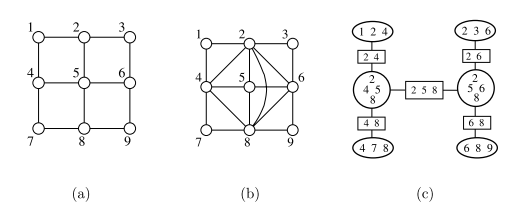
\includegraphics[width=.8\linewidth]{2-11.PNG}
    \caption{
        构建联合树的过程。
        (a) 原图是一个 $3 \times 3$ 的网格。
        (b) 原图的三角化版本。
        注意中间有两个 4-团。
        (c) 与 (b) 相对应的联合树,椭圆表示最大团,矩形表示分割子(Separator)。
    }\label{fig:2-11}
\end{figure}

原则上联合树算法的第三步中的推理可以在任意交换半环上执行(如我们之前在关于树算法的讨论中提到的)。
读者可以参考 Dawid 的作品,里面对最大积算法的联合树版本进行了广泛的讨论。
具体起见,我们在这里只讨论和积算法的联合树版本。
在联合树推断算法中通过在分割子——团结构之间的矩形(见图 \ref{fig:2-11})——上引入势函数而不仅仅只是在团结构上可以很优雅地表达基本的代数操作。
令 $\phi_C(\cdot)$ 代表在团结构 $C$ 上子向量 $x_C = (x_t, t \in C)$ 的势函数。
联合树上的团结构的势函数可以由原图的势函数获得。
分割子的势函数初始化为 1。
在此基础上可以给出联合树算法的基本消息传递步骤:
\begin{subequations}
\begin{align}
    \widetilde{\phi}_S(x_S) &\leftarrow \sum_{x_{B/S}}\phi_B(x_B) \\
    \phi_C(x_C) &\leftarrow \frac{\widetilde{\phi}_S(x_S)}{\phi_S(x_S)}\phi_C(x_C)
\end{align}
\end{subequations}
在连续的情况下求和可以用积分代替。
我们把这对操作称为“将消息从团 $B$ 传递到团 $C$”(如图 \ref{fig:2-12})。
可以验证一条消息如果从 $B$ 传递到 $C$ 再从 $C$ 传递到 $B$,结果彼此的团势是一致的,这意味着它们在节点集 $S$ 上是一致的。

\begin{figure}[htbp]
    \centering
    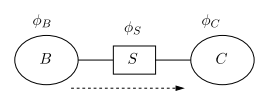
\includegraphics[width=.5\linewidth]{2-12.PNG}
    \caption{
        团 $B$ 和团 $C$ 之间通过分割子集 $S$ 的一次消息传递操作。
    }\label{fig:2-12}
\end{figure}

在联合树上经过一轮消息传递之后,可以看到整个联合树上团势与边际概率成正比。
也就是说,令 $\mu_C(x_C)$ 代表 $x_C$ 的边际概率,则有 $\mu_C(x_C) \propto \widetilde{\phi}_C(x_C)$。
这个性质可以通过对前面所介绍的和积算法的证明进行适当地推广得到(参见 Lauritzen 的作品)。
请注意,如果团势与边际概率是成比例的,那么每一对团结构之间满足局部的一致性显然是一个必要条件。
这就是运行交集性的意义所在,保证局部一致性蕴含全局一致性。

联合树算法有一个很重要的衍生结论,可以对分布 $p$ 表示成另外一种形式。
令 $\mathcal{C}$ 代表 $\widetilde{G}$ 中的最大团集合(也就是联合树中的节点),令 $\mathcal{S}$ 表示分割子的集合(也就是联合树中团结构之间的交集)。
要注意的是给定的分割子 $S$ 可能在联合树上出现很多次。
对于每个给定的分割子 $S \in \mathcal{S}$,设 $d(S)$ 表示其相邻的最大团的数目。
联合树框架使得分布 $p$ 可以按照下式进行因子分解
\begin{equation}
    p(x_1, x_2, \dots, x_m) = \frac{\prod_{C \in \mathcal{C}}\mu_C(x_C)}{\prod_{S \in \mathcal{S}}[\mu_S(x_S)]^{d(S)-1}}
\end{equation}
其中 $\mu_C$ 和 $\mu_S$ 分别代表团结构和分割子上的边际分布。
不同于因子分解式 (2.2),式 (2.12) 是直接以边际分布的形式来表达的,也不需要什么归一化常数(也就是说 $Z = 1$)。

\begin{tcolorbox}
\begin{exam}[马尔可夫链]
    考虑如下只包含三个变量的一个简单马尔可夫链 $p(x_1, x_2, x_3) = p(x_1)p(x_2|x_1)p(x_3|x_2)$。
    对应的图模型上的团包括 $\{1, 2\}$ 和 $\{2, 3\}$,之间的分割子为 $\{2\}$。
    很显然这个分布不能写成只包括团的边际的乘积。
    但是我们引入分割子之后就能写成下面这种边际形式:
    \[p(x_1, x_2, x_3) = \frac{p(x_1, x_2)p(x_2, x_3)}{p(x_2)}\]
    而且很容易验证这种边际的形式可以从式 (2.11) 导出,只需要设定 $\phi_{\{1, 2\}}(x_1, x_2) = p(x_1)p(x_2|x_1)$、$\phi_{\{2, 3\}}(x_2, x_3) = p(x_3|x_2)$。
\end{exam}
\end{tcolorbox}

为了给我们后续的内容做铺垫,考虑如下关于联合树表示的一种“反向”视角。
假设我们得到了一组关于联合树上团结构和分割子的函数 $\{\tau_C, C \in \mathcal{C}\}$ 与 $\{\tau_S, S \in \mathcal{S}\}$。
有哪些条件能够使得这些函数成为某种分布的有效边际?
假设这些函数在以下意义上是局部一致的:
\begin{subequations}
\begin{align}
    \forall S \in \mathcal{S}, &\sum_{x_S'}\tau_S(x_S') = 1 \\
    \forall C \in \mathcal{C}, S \subseteq C, &\sum_{\{x_C'|x_S' = x_S\}}\tau_C(x_C') = \tau_S(x_S)
\end{align}
\end{subequations}
上述联合树理论的本质是,这种局部一致性就是保证这些函数是某种分布的有效边际的充要条件。
为便于以后参考,我们将此结论做如下声明:
\begin{tcolorbox}
\begin{prop}
    函数组 $\{\tau_C, C \in \mathcal{C}\}$ 与 $\{\tau_S, S \in \mathcal{S}\}$ 可以作为联合树上团结构与分割子的边际分布当且仅当对于所有分割子 $S \in \mathcal{S}$ 都有归一化式 (2.13a) 从成立,且对于所有团结构 $C \in \mathcal{C}$ 都有边际化式 (2.13b) 成立。
    此外,所有满足这种局部一致性的函数都是由式 (2.12) 所定义的概率分布的边际。
\end{prop}
\end{tcolorbox}
这种联合树的表示形式将在我们后续的内容中发挥很大的作用。

最后我们讨论一下关于联合树算法计算复杂度的问题。
式 (2.11) 表明计算代价将随着联合树中最大团的规模呈指数增长。
显然人们感兴趣的就是控制团的规模。
图上所有潜在的三角形上的最大团的规模是一个重要的图论量,称为图的树宽\footnote{更准确地说,树宽是最大团的规模减一}。
因此,联合树算法的复杂度在树宽上呈指数级。

对于某些类型的图,例如链结构和树结构,树宽较小,联合树算法为推断问题提供了有效的解决方案。
很多著名的图模型架构都是如此,从中可以得到联合树算法的多种经典递归变体,包括计算遗传学中的剪枝和削皮算法,隐马尔可夫模型的前后向算法,状态空间模型的卡尔曼滤波算法等。
另一方面,也有许多图模型的树宽相当大,包括 2.4 小节中谈到的几个例子。
为了解决这种图模型必须放弃联合树框架,转而去寻找近似推断算法。

\section{近似推断的消息传递算法}

本书剩余部分的内容是提出一种近似计算边际分布和似然以及整数规划的变分方法理论框架。
这样做需要凸分析和指数族的数学背景知识,我们将在第三章中提供。
然而从历史上看,许多算法是在没有这些背景的情况下发展起来的,它们依赖的是物理直觉或者是对精确或近似蒙特卡洛算法的类比。
在本节中我们将对两种变分推断算法的这种特性进行高层次的描述,以突出它们的简单和直观性质。

我们考虑的第一个变分算法是应用于带环图的和积消息传递,被称为“循环的(Loopy)”和积算法或者信念传播算法(Belief propagation)。
回想一下,和积算法是树结构的精确推断算法,然而但从算法的角度上来说,当然也可以尝试将它应用到带环图上。
更具体地说,消息更新式 (2.9) 可以在给定的节点上运行,忽略环的存在就行。
直观上来讲,如果图比较稀疏或者存在某种特殊的对称性,这样的算法可能可行,因为在环上传播的影响会比较小。
正如 2.4 小节中讨论的,该算法实际上已经成功地获得了很多的应用。
此外,最大积算法的一种类似形式也可以用来计算带环图上的近似众数。

第二种变分算法就是所谓的朴素平均场算法(Naive Mean Field)。
我们将会描述该算法在 Ising 模型中的应用,这是一个包含二元随机向量 $X \in \{0, 1\}^m$ 的无向图模型或者马尔可夫随机场,其中相邻节点对有一个耦合权重 $\theta_{st}$,每一个节点还有一个观测权重 $\theta_s$。
(关于该模型的详细描述参见 3.3 解的例 3.1。)
为了给朴素平均场提供一些直观认识,我们首先在这个特殊的模型上描述吉布斯采样(Gibbs Sampler),这是一种特殊类型的 MCMC 算法。
吉布斯采样的基本步骤是随机选择一个节点 $s \in V$,然后在邻居状态固定的情况下,根据条件概率更新相关随机变量的状态。
更准确地说,令 $N(s)$ 表示节点 $s \in V$ 的邻居,令 $X_{N(s)}^{(n)}$ 代表节点 $s$ 的邻居在第 $n$ 次迭代时的状态,则节点 $s$ 的状态更新如下
\begin{equation}
    X_s^{(n+1)} = \begin{cases}
        1 & \text{如果} U \leq \{1 + \exp{[-(\theta_s + \sum_{t \in N(s)}\theta_{st}X_t^{(n)})]}\}^{-1} \\
        0 & \text{其他}
    \end{cases}
\end{equation}
其中 $U$ 为采样自均匀分布 $\mathcal{U}[0, 1]$ 的一个样本。

在稠密图中,这样的邻居集合 $N(s)$ 的基数可能很大,我们可以尝试使用大数定律或者其他计算方式来估计 $\sum_{t \in N(s)}\theta_{st}X_t^{(n)}$。
就这个求和的稠密程度而言,用期望代替样本值可能比较有效。
也就是说,令 $\mu_s$ 代表每个节点 $s \in V$ 边际概率 $\mathbb{P}[X_s = 1]$ 的一个估计值,我们可以考虑式 (2.14) 的一个平均形式:
\begin{equation}
    \mu_s \leftarrow \{1 + \exp{[-(\theta_s + \sum_{t \in N(s)}\theta_{st}\mu_t)]}\}^{-1}
\end{equation}
因此与其依赖其邻居状态的条件概率更新随机变量 $X_s$,不如确定性地更新一个参数 $\mu_s$,它也依赖于其邻居的相应参数。
式 (2.15) 定义了 Ising 模型的朴素平均场算法。
与和积算法一样,平均场算法也可以看作是一种消息传递算法,式 (2.15) 右边表示到达节点 $s$ 的“消息”。

乍一看这种消息传递算法似乎还有些问题。
算法会导致不动点吗?
算法会收敛吗?
本书剩下的内容就是对这些问题进行讲解。
最终我们将看到一大类消息传递算法,包括平均场算法、和积算法、最大积算法,以及这些方法的各种拓展,都可以被理解为变分问题的精确或者近似的版本。
指数族和凸分析是下一章的主题,它们提供了一种统一的框架来发展这些变分原理。


